\subsection{SD-Karte}\label{sec:sdKarte}
Um auf die SD-Karte zuzugreifen, wurde die Library fatfs verwendet. Sie ermöglicht einen einfachen Zugriff auf die Daten per SPI-Schnittstelle. Sie wird im ersten Kapitel beschrieben, anschliessend behandelt ein Kapitel die Bündelung des Codes in Zusammenhang mit der SD-Karte. Darum wurde ein eigenes Modul geschrieben. Das letzte Kapitel beschreibt noch die benötigten Files auf der SD-Karte um die Funktionen des Dōjō zu gewährleisten.

\subsubsection{fatfs}
Loosli?

\subsubsection{SD-Karte Modul}
Anschliessend sind die verschiedenen Funktionalitäten aufgelistet.

\subsubsection*{Merken}
Das Modul beinhaltet zwei Funktionen um die Funktionalität des Merken zu realisieren. Die Erste speichert das aktuelle Kunstwerk auf eine Liste. Auf dieser Liste werden die verschieden gemerkten Kunstwerken gesammelt. Die zweite Funktion löscht eben diese Liste wieder, um den Dōjō bereit für den nächsten Nutzer bereit zu machen. Den Dateinamen der Liste lässt sich im Header-File anpassen.

\subsubsection*{SD-Karte Initialisieren}
Diese Funktion ruft eine Reihe fatfs-Befehle auf um die SD-Karte zu mounten. Diese wird über ein SPI-Bus an den Microkontroller angeschlossen. Die Pins für den Bus lassen sich im Header-File definieren.

\subsubsection*{Lookup}
Diese Funktion ist die eigentliche Implementierung des in Abbildung \ref{fig:lookupState} beschrieben Algorithmus.

\subsubsection*{Sprachwechsel}
Diese Funktion wechselt die Sprache des Dōjō. Die Sprachauswahl geschieht über verschiedene Files. Es exisitert für jede Sprache ein eigenes Lookup-File. Dieses verbindet die Majo-Minor-Kennzeichnungen mit den Wav-Files der jeweiligen Sprache. Dadurch muss für einen Sprachwechsel nur der Zeiger auf das Lookup-File geändert werden.

\subsubsection{Benötigte Files}
Im Header-File des Moduls SD-Karte müssen verschiedene Files definiert werden. Diese müssen auch auf der SD-Karte vorhanden sein und im richtigen Format. Die Merken-Liste ist eine normale .txt Datei. Sie sollte leer sein. Des weiteren müssen die Lookup-Files vorhanden sein. Sie sollten dem in Abbildung \ref{fig:definition_lookup_file} definierten Format entsprechen. Zu beachten ist, dass die X Symbole für zwei stellige Hex-Zahlen stehen. Somit hat es eine Referenz auf ein Kunstwerk pro Zeile.

\begin{figure}[H]
	\begin{center}
		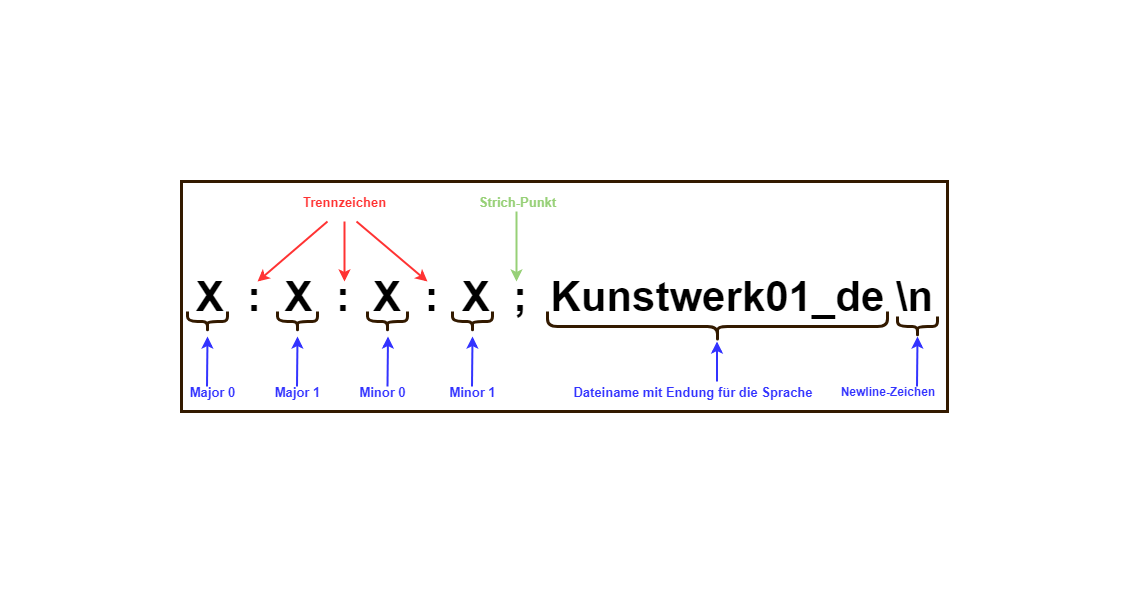
\includegraphics[width=140mm]{data/Definition_picture.png}
		\caption[Formatdefinition Lookup-File]{Formatdefinition Lookup-File} %picture caption
		\label{fig:definition_lookup_file}
	\end{center}
\end{figure}

Wav files Loosli?

